\documentclass[final]{anthology-ch}

\ExecuteBibliographyOptions{maxcitenames=99,maxbibnames=99}

\usepackage{booktabs}
\usepackage{graphicx}

\usepackage{booktabs}
\usepackage{tabularx}
\usepackage{longtable}
\usepackage{array}
\usepackage{caption}
\usepackage{adjustbox}

\title{Authorial Filtering and Computational Models: A Dynamic Analysis of Umberto Eco's \textit{Foucault's Pendulum} through a Fluid-Dynamics-Inspired Framework}

\author[1]{Lorenzo Zangari}[
orcid=0009-0009-9057-1299
]

\author[1]{Davide Picca}[
orcid=0000-0003-2014-0855
]

\author[2]{Riccardo Fedriga}[
orcid=0000-0002-2291-7800
]

\affiliation{1}{SLI, University of Lausanne, Lausanne, Switzerland}

\affiliation{2}{DAR, University of Bologna, Bologna, Italy}

\keywords{PLMs, Fluid-dynamics, Computational narratology}

\pubyear{2025}
\pubvolume{3}
\pagestart{1107}
\pageend{1120}
\conferencename{Computational Humanities Research 2025}
\conferenceeditors{Taylor Arnold, Margherita Fantoli, and Ruben Ros}
\doi{10.63744/yVYI1Je9wQvM}
\paperorder{65}

\addbibresource{bibliography.bib}

\newcommand{\spara}[1]{\vspace{0.1cm}\noindent{\bf #1}}
\newcommand{\src}{\textsf{SRC}}
\newcommand{\mxr}{\textsf{}{MXR}}
\newcommand{\snk}{\textsf{SNK}}

\newcommand{\refapp}[1]{Appendix~\ref{app:#1}}

\begin{document}

\maketitle
\begin{abstract}
Authorial-filtering plays a crucial role in constructing literary meaning. It is the narrative act of selectively activating, suppressing, or leaving certain information latent within a story. Umberto Eco's Foucault's Pendulum stands as a paradigmatic case of this phenomenon, as it exemplifies  a narrative  wherein presence and absence, action and potentiality, remain in constant flux through intra- and intertextual interplay. In this preliminary study, we propose a novel computational framework inspired by fluid dynamics to detect authorial-filtering information within literary texts. Applying this approach to Foucault's Pendulum, our results reveal how narrative motifs and topics flow, diffuse, and react throughout the text, closely mirroring the qualitative interpretations of domain experts. Our proposed framework not only sheds new light on Eco’s complex narrative mechanisms but also advances computational narratology by providing an interpretable model for digital literary analysis. We make the implementation of our framework publicly available.\footnote{\url{https://github.com/lorenzozangari/fluid-dynamics-af}}
\end{abstract}

\section{Introduction}

Understanding fiction presents a unique challenge: fictional narratives, and especially novels, demand that readers engage with complex, layered meanings rooted in imaginative ontologies. For instance, analyzing Sherlock Holmes’s 221b Baker Street---even as a fictional construct---reveals how narrative objects transcend mere real-world descriptions. The address works within the story despite being fictional, showing that fictional worlds operate by internal logic, not real-world correspondence. Within such worlds, readers must suspend disbelief and navigate higher-order entities, a process that often surpasses the capacity of standard computational heuristics \cite{Fedriga2023a}. This interpretation effort links object traits to author intent through narrative structure.

At the heart of this negotiation lies what Eco has termed \emph{authorial-filtering}: the process through which meaning emerges via selective narrative acts, such as transformation, or emphasis, that shape reader expectations \cite{Eco1990}. Unlike simple data projection, formal analysis in this context is an \emph{intensional} mapping of authorial actualization \cite{Eco1997,Sperber1995}. Therefore, any computational model of fiction should represent evolving higher-order objects by balancing extensional data and intensional interpretation, while also accommodating the inherent structural evolution of the text \cite{Eco2023b,Domenella2025}.

Recent advances in \emph{Natural Language Processing (NLP)}, and especially the development of \emph{Pre-trained Language Models (PLMs)} \cite{min2023recent}, have dramatically enhanced our ability to analyze textual data \cite{zangari2025survey}. However, PLMs struggle with authorial-filtering, as this process depends on detecting discrete, context-sensitive narrative choices that are deeply embedded in literary structure \cite{subbiah2024reading}. This challenge is illustrated by works such as \emph{Foucault’s Pendulum}, where presence and absence, action and potentiality are interwoven in recursive, intertextual patterns that produce a narrative pact of excess and omission, often evoking a conspiratorial atmosphere \cite{Brotherton2017}.

Our preliminary study addresses the above challenges by proposing a novel framework inspired by fluid dynamics. Specifically, we adapt the concepts of \emph{advection, diffusion, and reaction} to simulate the evolution and flow of narrative units throughout a literary text. This approach is motivated by recent research that has successfully applied \emph{advection-diffusion-reaction (ADR)} models to phenomena outside classical fluid dynamics: for example, modeling road density as a flowing fluid \cite{kumar2023urban} or the spread of disease in populations \cite{cheng2023epidemic}. Closely related to our work is the use of ADR to represent lexical density and emotional dynamics within literary texts \cite{picca2024fluid}. In the ADR framework, advection transports quantities in a preferred direction, diffusion spreads and smooths those quantities, and reaction either injects or removes them from the system \cite{Ellery2012critical}.

Applying this intuition to literary analysis, we treat \emph{narrative paragraphs} (hereafter, paragraphs) as the atomic units of fictional narrative. Defined by specific narrative parameters, such as location, objects, and the involved characters, these units structure the story’s context, capturing both explicit and latent information.
We then frame narrative filtering as a set of dynamic processes in which textual entities and motifs experience activation, latency and, transformation phases directly analogous to those found in fluid dynamics. Narrative meaning depends as much on concealment as on disclosure,  thus  effective models must intertextually trace how themes, characters, and spaces appear or vanish across the paragraphs.  To the best of our knowledge, this is the first fluid-dynamic-inspired computational framework designed  to detect authorial-filtering in literary analysis.

We summarize our key contributions as follows: (i) we formally define the authorial-filtering task in literary texts; (ii) we propose a novel conceptualization of authorial-filtering through a fluid-dynamic approach, highlighting narrative choices via the detection of latent narrative units that emit or absorb new material; and (iii) we interpret the resulting patterns with computational and humanistic evidence, validating the framework’s coherence with the novel.

\section{Methodology}
\begin{figure}[t]
\centering
\includegraphics[width=1.0\linewidth]{figures/overview.png}
\caption{Overview of our fluid-dynamic-inspired framework.
}
\label{fig:overview}
\end{figure}

\spara{Problem statement.} We aim to detect the authorial-filtering map within the novel, i.e., the selective choices the author makes among all possible narrative parameters. This entails tracing the introduction, persistence, and withdrawal of such parameters to measure their functional consumption. Formally, let \(\mathcal{B}\) denote a corpus and \((P_1,\dots,P_n)\) be its temporally ordered sequence of paragraphs. For each paragraph \(P_i\), let \(\mathbf{Q}_i\) be the vector of its local narrative parameters (e.g., a character involved in the novel). Our goal is to produce
a filtering vector $\mathbf{F} \in \mathbb{R}^{n}$, where its $i$-th component, $F_i$, quantifies the intensity of the author’s filtering intervention on paragraph $P_i$ and $\operatorname{sgn}(F_i)$ indicates the direction of the intervention.

\spara{Overview.} Figure \ref{fig:overview} illustrates the conceptual architecture of our approach. Given a corpus $\mathcal{B}$ and a corresponding ontology $\mathrm{T}$, we first segment the text into paragraphs as dictated by the author’s style. We then extract narrative parameters and linked them to the esoteric domain framed by the ontology.  From this paragraph-level segmentation and the associated narrative parameters, we computed each paragraph’s initial state as its relative strength across ontological classes. Finally, we constructed a literary-plot graph and used it as a medium for an advection-diffusion-reaction simulation. The steady-state solution yields the vector $F$ representing the authorial-filtering process.
In the following, we first formalize the problem and describe each module of our framework.

\spara{Paragraph segmentation.} Paragraph segmentation is performed by splitting the corpus at either double newlines, commonly used to denote paragraph boundaries, or at sequences of four or more consecutive spaces, which typically appear in plain-text formats to simulate vertical spacing or mark structural breaks. In fact, Eco uses visible paragraph breaks to signal shifts in argument or semiotic perspective in his novels \cite{eco2017come}.

\spara{Narrative parameters detection.} To detect narrative parameters, we used a Named Entity Recognition (NER) model, which identifies expressions in natural language that denote named entities, such as people, places, and organizations, and classifies them into predefined categories. In our specific scenario, labels such ORG denotes  institutions (e.g., Union of Industrialist), and LOC refers to physical locations (e.g., Milan).
Examples of narrative parameters are shown in \refapp{appner}.

\spara{Graph of literary plots}. In this study, we employed a graph of literary plots $G$ (see \refapp{literary_plot}) that connects each paragraph to its most semantically and temporally similar paragraphs. Specifically, edges are weighted through the cosine similarity of sentence embeddings. To avoid noisy connections, only the
top-$r$ most similar paragraphs are linked, provided that their similarity score exceeds the threshold $\tau$.

\spara{Ontological strength estimator.}
A literary graph can also be analyzed using standard network algorithms \cite{chung2014brief}.
Nevertheless, such methods are intrinsically static and limited in their ability to determine authorial-filtering. To overcome this limitation, we treated the graph as a hydraulic network in which each node stores an initial intensity, that is, the local concentration of meaning. Formally, let \(\mathsf{T}=(\mathcal{C},\mathcal{A})\) be an ontology, with \(\mathcal{C}=\{C_1,\ldots,C_m\}\) and $\mathcal{A}$ is the set of assertions (ABox).
To estimate the relevance of a paragraph $P_i$ with respect to a class $C_j$, we introduce a strength function $s : \mathcal{P} \times \mathcal{C} \rightarrow [0,1]$, given by: (i) a \emph{lexical score} $s_{\mathrm{lex}}$, which measures the affinity between the paragraph’s narrative-parameter vector and the class taxonomy; and (ii) a \emph{contextual score} $s_{\mathrm{ctx}}$, which captures contextual and semantic information. Their computation, based on PLMs, is defined in \refapp{lex_sem}.
The final score $s$ is obtained using the following convex combination:

\begin{equation}\label{eq:init_score}
s(P_i,C_j) = \alpha s_{\text{lex}} + (1-\alpha) s_{\text{ctx}},
\end{equation}

\noindent

where $\alpha \in [0,1]$ is the importance of the lexical component.

\spara{Fluid-dynamic-inspired simulation.}
To model authorial-filtering, we consider the semantic graph as a hydraulic network, where each node (i.e., paragraph) is initialized with a ``pressure'' value $S^{(0)}_{i,j} = s(P_i, \mathcal{C}_j)$. An ADR-based simulation evolves these values over time, yielding at each time step \(t\) the quantity \(S_{i,j}^{(t)}\), which denotes the intensity of the signal in paragraph \(P_i\) for class $\mathcal{C}_j$ at simulation time \(t\). The propagation equation is given by Eq. \ref{eq:adr}:
\begin{equation}\label{eq:adr}
\begin{split}
\underbrace{S_{i,j}^{(t)}}_{\text{storage term}}
&=
\underbrace{-\sum_{k\;:\;(i,k)\in E} w_{ik}\,\bigl(S_{i,j}-S_{k,j}\bigr)}_{\text{advection}}
\;+\;
\underbrace{\nu \sum_{k\in\mathcal N_i} \bigl(S_{k,j}-S_{i,j}\bigr)}_{\text{diffusion}}
\\[4pt]
&\quad+\;
\underbrace{\lambda_{\mathrm{inj}}\,\sum_{k\;:\;(i,k)\in E} w_{ik}\,\bigl(S_{i,j}-S_{k,j}\bigr)
\;-\;
\lambda_{\mathrm{dec}}\bigl(S_{i,j}-S^{(0)}_{i,j}\bigr)}_{\text{reaction}}.
\end{split}
\end{equation}

The storage term measures the instantaneous variation in the narrative pressure. $\mathcal{N}_i$ is the neighbor set of $P_i$;
$w_{ik}$ denotes the edge velocity.
A positive \(w_{ik}\) advects the thematic mass from \(i\) to \(k\), whereas a negative value reverses the flow.  $\nu$ is the viscosity term, indicating how rapidly the diffusion term decreases.
\(\lambda_{\text{inj}}\) boosts the value of selected paragraphs, while \(\lambda_{\text{dec}}\) drives a relaxation toward the baseline value $S_{i,j}^{(0)}$. Their combination acts as a self-regulating term, limiting growth without hindering advection-diffusion. Finally, Equation~\eqref{eq:adr} is solved using a two-stage explicit Runge-Kutta (Heun) scheme \cite{butcher2016numerical}.  The procedure stops when the median relative change falls below the threshold $\eta$. The final output is $\mathbf{S}^{\ast}_i \in \mathbb{R}^{k}$, which indicates the steady-state strength vector for paragraph $P_i$.

\spara{Subtractive filtering.}
We obtained the authorial-filtering vector by filtering out paragraphs that did not contribute to the narrative dynamics.  Specifically, we evaluated, for each $P_i$, the net advective flux:

\begin{equation}
\Delta_i \;=\; \sum_{j=1}^{k}\sum_{(i,k)\in E} w_{ik}\,\bigl(S^{\ast}_{i,j}-S^{\ast}_{k,j}\bigr),
\end{equation}

\noindent

where \( S^{\ast}_{i,j} \) denotes the steady state of class \( \mathcal{C}_j \) at \( P_i \) after the propagation convergence. An adaptive threshold \( \mu \) is defined as the first quartile of \( |\Delta| \).
Based on the value of \( \Delta_i \), each paragraph is assigned to one of three categories, reflecting its role in the flow of narrative themes:

\begin{itemize}
\item \textbf{Source paragraphs (\src):} If \( \Delta_i < -\mu \), the paragraph is considered a \emph{source}. This means it introduces or releases new narrative elements into the story, acting as a point of origin from which ideas, themes, or motifs begin to spread to other parts of the text.

\item \textbf{Sink paragraphs (\snk):} If \( \Delta_i > \mu \), the paragraph is categorized as a \emph{sink}. In this case, the paragraph absorbs or collects narrative content; themes or ideas that have circulated earlier in the text tend to be resolved, closed, or absorbed here.

\item \textbf{Mixer paragraphs (\mxr):} If \( |\Delta_i| \leq \mu \) and the advective flux dominates over diffusion, the paragraph is labeled as a \emph{mixer}. They are transition points where multiple ideas or themes meet and interact, but without merging into a single coherent thread. Instead, they hold different narrative elements in tension, allowing the story to shift perspective or tone.
\end{itemize}

Then, to represent the fact that the author has reversed the thematic flow, for example, turning an injection into a drainage or vice versa, we define the residual field \(\mathbf{R}_i = \mathbf{S}^{\ast}_i - \mathbf{S}^{(0)}_i\). We
retain only those values corresponding to  two consecutive paragraphs that change roles (e.g., $P_{i-1}$ is \src{} and $P_i$ is a \snk). Summing the retained \(R_{i,j}\) yields the filtering score \(F_i\), which quantifies the filtering decisions, as shown in Eq. \ref{eq:finale}.

\begin{equation}\label{eq:finale}
F_i = \sum_{j=1}^{k}
\mathbb{I}\bigl[\operatorname{sign}(R_{i-1,j}) \neq \operatorname{sign}(R_{i,j})\bigr]\,
R_{i,j},
\end{equation}

\noindent

where $\mathbb{I}$ is the indicator vector and the final filtering vector is $\mathbf{F} = \bigl[F_1,\dots,\,F_{|\mathcal{P}|}\bigr]^{\!\top}$. A negative \(F_i\) indicates that the paragraph injects more themes than it receives, whereas a positive \(F_i\) indicates that the paragraph receives more themes than it injects.

\section{Experimental evaluation}

\spara{Evaluation goals.}  We designed our experimental evaluation to evaluate the coherence of the steady-state vector computed by our computational model and to detect the authorial-filtering information within specific chapters of Umberto Eco's Foucault Pendulum.  The experimental setting is reported in \refapp{experimental}.

\spara{Data.} We used the ontology $\mathrm{T}$ shown in \refapp{appendix_onto}, with the following classes:  \emph{Concepts}, \emph{Traditions}, \emph{Languages and Codes}, and \emph{Figures and Archetypes}.
We manually populated the ontology with assertions retrieved in the first four Chapters of the novel  ($158$ paragraphs out of $700$).

\subsection{Results}

\begin{figure}[t]
\centering
\includegraphics[width=1.0\linewidth]{figures/heat_map.png}
\caption{Steady state profile of paragraphs with respect to each top-level concepts. Dashed white lines mark the end of one Chapter and the beginning of the next.
}
\label{fig:heatmap}
\end{figure}
\spara{Assessment of the steady state profile.} We qualitatively assessed the steady-state vectors $\mathbf{S}^{\ast}_{i}\in\mathbb{R}^{k}$ for each paragraph $P_i\in P$, representing the final distribution of top-level concept intensity after the ADR dynamics reach equilibrium on the similarity–temporal graph.

Figure~\ref{fig:heatmap} shows a heatmap where the color intensity reveals how much each paragraph develops one of the text’s main conceptual categories (\refapp{appendix_onto}). The more intense the color, the more that particular idea appears in that part of the narrative as expressed by the steady-state vectors $\mathbf{S}^{\ast}_{i}\in\mathbb{R}^{k}$.
For the theme \emph{Concepts}, the color remains fairly constant throughout the novel. This means that references to symbolism and hidden knowledge are sprinkled everywhere, often present but never concentrated in just one place. Instead of sharp peaks, the model finds many small and frequent hints spread across the text, thereby creating a flat profile.
Examining the macro-category \emph{Traditions}, we observe a clear pattern of alternating bands, corresponding to deliberate narrative shifts, as the text cycles between phases of emphasis and retreat on esoteric traditions. The heightened values in certain segments signal points in the story where references to traditions become particularly salient, while the lighter areas mark narrative stretches in which these themes recede into the background. This behavior closely follows the changing focus of the plot, confirming that the model effectively captures the dynamic presence and contextual reactivation of the theme of tradition throughout the early chapters of the novel.
By contrast, the \emph{Figures and Archetypes} line features distinct spikes, particularly near paragraphs 25, 66–69, 120, and 139. These correspond to the narrative’s explicit focus on emblematic figures such as the \emph{Count of Saint-Germain}, \emph{Hugh de Payns}, \emph{Cagliostro}, and \emph{John Dee}. In these passages, the narrative focuses almost exclusively on a specific character.
Turning to \emph{Languages and Codes}, the signal is strong at the beginning, driven by discussions of Abulafia’s combinatorial Kabbalah and early cipher lore, and rises again during the library scene, where coded devices such as Trithemius’s rotulae, quadratic diagrams, and magic squares are explored in detail. This demonstrates that numerical or mathematical imagery, by itself, does not suffice; what matters is that these elements are framed by an explicit cryptographic discourse.
In short, peaks in the heatmap align with paragraphs that introduce new ritual, historical, or cryptographic content, while troughs appear in connective passages that absorb or link existing themes without adding anything genuinely new. This suggests that the model is sensitive to real content shifts, rather than merely smoothing over noise.

\begin{figure}[t]
\centering
\includegraphics[width=1.0\linewidth]{figures/auth_1.png}
\caption{Authorial-filtering diagram of Umberto Eco's Foucault Pendulum up to Chapter 4. \(P_i (c_i)\) represents the paragraph number and the corresponding Chapter. Green, red and orange blocks represent \src{}, \snk{} and \mxr{} paragraphs, respectively; purple- and blue-colored blocks indicate narrative parameters and top-level categories of the ontology $\mathrm{T}$; $\infty cat$ denote a concept that is left open by the author, possibly for a later reactivation.}
\label{fig:authorial}
\end{figure}

\spara{Assessment of the authorial-filtering information.}
To effectively describe authorial-filtering, we display the narrative parameters linked to \src{}, \mxr{}, and \snk{} paragraphs, as depicted in Figure~\ref{fig:authorial}.
\src{} nodes emit more narrative material than they receive; they seed parameters that later reappear elsewhere (e.g., the first encounter with the Pendulum).
\snk{} nodes absorb or refract existing themes; they close threads or re-contextualize objects.
In \mxr{} nodes, multiple ideas co-exist without merging, producing abrupt shifts in perspective, such as digressions that place heterogeneous theories side by side. Blue blocks denote the top-level classes of $\mathrm{T}$, and $\infty cat$ denotes narrative hooks that the author leaves open for future use.

Looking at Figure~\ref{fig:authorial}, several remarks stand out.
In $P_{7}$, the Pendulum prompts \textit{Jacopo Belbo} to envision an embryonic universal “Plan.”
The diagram also shows that this concept remains active until Chapter 4 (no \snk{} nodes are associated with the Pendulum).
Belbo, a key character in the novel, appears in multiple branches.
He appears in $P_{23}$ as a \snk{} paragraph, where he suspects that the “Plan” may be only a game, draining meaning from earlier hypotheses:
He is reactivated in $P_{25}$, where new threats and actions spring from his perspective.
In $P_{117}$ (\mxr{}), Belbo receives De Angelis’s letter; personal intimacy, investigative reserve, and memories of the Plan run side by side without merging, forcing the reader to switch the tone repeatedly.

Paragraph $P_{94}$ introduces the apocalyptic triad \emph{Beast–Jerusalem–Anti‑Jerusalem}.
Three green source edges indicate a symbolic injection, whose effects propagate through the rest of the corpus. Jerusalem had appeared earlier in $P_{67}$ as a \snk{} paragraph: Here, the reference is strictly retrospective, as the Templars’ foundation and Baldwin II’s Jerusalem are summarized by one character.
No new material is projected forward; the section merely absorbs the circulating content.
This pattern shows Eco’s authorial filter: the motif is quarantined when the discourse needs consolidation ($P_{67}$) and later reactivated as an eschatological pivot ($P_{94}$).

Considering the sequence $P_{104}$–$P_{105}$, where \emph{Rakosky} appears as a \mxr{} and \src{}, respectively, Eco first holds heterogeneous ideas in suspension without advancing or concluding them,  then propagates them into a more complex set of possibilities. In $P_{104}$,
Belbo summarizes what was already told about \emph{Rakosky}.
In $P_{105}$, \emph{Rakosky} is no longer a mere mention, but drives several fresh investigative threads that radiate to other paragraphs, such as the Paris follow-up and the search for the missing dossier. Thus, this paragraph converts prior static information into outward-spreading, active narrative lines.

Multiple sources (Rosicrucian, Brazil, Easter) converge on \emph{Traditions} and \emph{Concepts}, which ultimately channel into the $\infty cat$ block, meaning that their last links are not connected to any \snk{} paragraph.
Considering \emph{Figures and Archetypes}, only \emph{Amparo} survives the filter, as it is mentioned more than twice in a single paragraph.
This indicates a state of latency because the narrative leaves different branches open. This behavior is expected because the model was run until Chapter 4. No parameters from the \emph{Languages and Codes} category were detected, likely because, up to Chapter 4, these parameters are absent from \src{}, \snk{}, and \mxr{} paragraphs.

Overall, Eco stores motifs in early sinks (e.g., Jerusalem in $P_{67}$), reactivates them later as strong sources (e.g., $P_{94}$), while initial seeds, such as the Pendulum in $P_{7}$ remain active and continue to propagate.
Thus, the diagram captures the narrative economy that regulates the introduction and circulation of themes.

\section{Conclusion}

This preliminary study showed that applying a fluid-dynamics-inspired model to authorial-filtering provides an interpretive key to the dynamic complexity of Eco’s narrative. The mapping of \src{}, \snk{} and \mxr{} paragraphs reveals how Eco orchestrates the circulation of themes, symbols, and characters through non-linear patterns, confirming the recursive and processual nature of meaning-making in the novel. The fluid dynamics analogy proves productive: the activation, latency, and re-emergence of semantic nuclei are not only traceable but also become visible indicators of the author’s strategies of dissemination and concealment, suggesting that narrative functions as a semiotic ecosystem in constant transformation.

The identified limitations, such as the difficulty in capturing certain narrative parameters or the need for greater ontological richness (e.g., the \emph{Language and Codes} classes was not detected), highlight how essential it is to integrate computational and humanistic approaches to truly grasp literary complexity. Therefore, this study not only confirms the validity of the proposed model but also points to future developments, both methodologically (with more sophisticated semantic network extraction) and theoretically, paving the way for a computational narratology able to model not just data, but the very conditions under which literary meaning emerges.

\printbibliography

\appendix

\section{Notations}\label{app:notations}

Table \ref{tab:notation} lists the notations used throughout this study.

\begin{table}[t]
\centering
\caption{Notation used throughout the paper}
\begin{tabularx}{0.8\textwidth}{@{}lX@{}}
\toprule
\textbf{Symbol} & \textbf{Description}\\
\midrule

$i,k$ & Index of paragraphs (\(P_i\))\\
$j$ & Index of ontological classes (\(C_j\))\\
$n$ & Total number of paragraphs in the corpus \(B\)\\
$m$ & Total number of ontological classes\\
\midrule

$\mathcal{B}$ & Corpus (Umberto Eco’s \emph{Foucault’s Pendulum})\\
$\mathcal{P}=(P_1,\dots,P_n)$ & Ordered sequence of paragraphs\\
$P_i$ & \(i\)-th paragraph (minimal narrative “basin”)\\
$Q_i\in\mathbb{R}^d$ & Narrative‑parameter vector extracted from \(P_i\)\\
$G=(V,E,W)$ & Directed weighted literary–plot graph\\
$V$ & Node set of \(G\) (paragraphs)\\
$E$ & Edge set of \(G\) (narrative links)\\
$W:E\!\to\!\mathbb{R}_{\ge0}$ & Edge‑weight function (link strength)\\
$w_{i,k}$ & Weight / advective velocity on edge \((i,k)\)\\
$\mathcal{N}_i$ & Neighbour set of \(P_i\) in \(G\)\\
\midrule

$T=(\mathcal{C},\mathcal{A})$ & Esoteric ontology: classes \(\mathcal{C}\), A‑box \(\mathcal{A}\)\\
$\mathcal{C}=\{C_1,\dots,C_m\}$ & Set of ontological classes\\
$C_j$ & \(j\)-th ontological class\\
$\mathcal{A}_{C_j}$ & A‑box fragment instantiating \(C_j\)\\
$s(P_i,C_j)$ & Composite strength of paragraph \(P_i\) for class \(C_j\)\\
$s_{\mathrm{lex}}$ & Lexical component of the strength score\\
$s_{\mathrm{ctx}}$ & Contextual / semantic component of the strength score\\
$\alpha\in[0,1]$ & Mixing coefficient in Eq.\,(1) for \(s_{\mathrm{lex}}\) and \(s_{\mathrm{ctx}}\)\\
\midrule
$S^{(t)}_{i,j}$ & Pressure after \(t\) ADR iterations\\
$S^{*}_{i,j}$ & Steady‑state pressure (converged value)\\
$\nu$ & Viscosity / diffusion coefficient\\
$\lambda_{\mathrm{inj}}$ & Injection coefficient in reaction term\\
$\lambda_{\mathrm{dec}}$ & Decay coefficient in reaction term\\
\midrule
$\Delta_i$ & Net advective divergence at paragraph \(P_i\)\\
$\mu$ & Adaptive threshold (first quartile of \(|\Delta|\))\\
$\mathrm{SRC}$ & \emph{Source} paragraphs: \(\Delta_i<-\mu\) (inject themes)\\
$\mathrm{SNK}$ & \emph{Sink} paragraphs: \(\Delta_i>\mu\) (drain themes)\\
$\mathrm{MXR}$ & \emph{Mixer} paragraphs: high advection, \(|\Delta_i|\le\mu\)\\
$R_i$ & Residual vector \(S^{*}_{i}-S^{(0)}_{i}\) for paragraph \(P_i\)\\
$F=(F_1,\dots,F_n)$ & Authorial-filtering vector\\
$F_i$ & Filtering score attached to paragraph \(P_i\)\\
\texttt{sgn}$(\cdot)$ & Sign operator \\
$\mathbb{I}[\cdot]$ & Indicator function (1 if condition holds, 0 otherwise)\\
\midrule
$r$ & Top‑\(r\) nearest neighbours kept per paragraph\\
$\tau$ & Similarity threshold for edge creation\\
$d$ & Minimum frequency of a narrative parameter within a paragraph\\
$\eta$ & Convergence tolerance for the ADR solver\\
\bottomrule
\end{tabularx}
\label{tab:notation}
\end{table}

\section{Umberto Eco's Foucault's Pendulum}\label{app:ecos}
Foucault’s Pendulum follows three Milanese editors who, jokingly, piece together myths, symbols and historical events into a grand conspiracy they dub ``The Plan.'' This fictional code links Templar legends to Renaissance alchemy, creating a labyrinthine network of literary and historical references. The novel’s layered narrative obscures the line between fact and fiction, compelling readers to question every connection. Analyzing this novel is useful for testing computational models’ ability to detect authorial intent and separate meaningful structures from constructed illusions.

\section{Advection-Diffusion-Reaction framework}\label{app:why}
Figure \ref{fig:why} depicts the ADR framework used in this study.

\section{Literary plot graph}\label{app:literary_plot}
To capture narrative structure information through inter-paragraph relationships, we adopt a graph-based model, which is widely used in digital humanities to represent narrative dynamics~\cite{chambers2008unsupervised, elson2010extracting}.
Specifically, we define a \emph{literary plot graph} as a directed weighted graph $G=(V,E,W)$ where $V$ are the nodes (i.e., paragraphs), $E\subseteq V\times V$ are the edges, and $W : E \rightarrow \mathbb{R}^+$ (i.e., relationships between paragraphs) is a weight function representing the strength of narrative relationships. Given two nodes $i$ and $k$, we denote the weights between them as $w_{ik}$, where $i,k \in E$.

\begin{figure}[!ht]
\centering
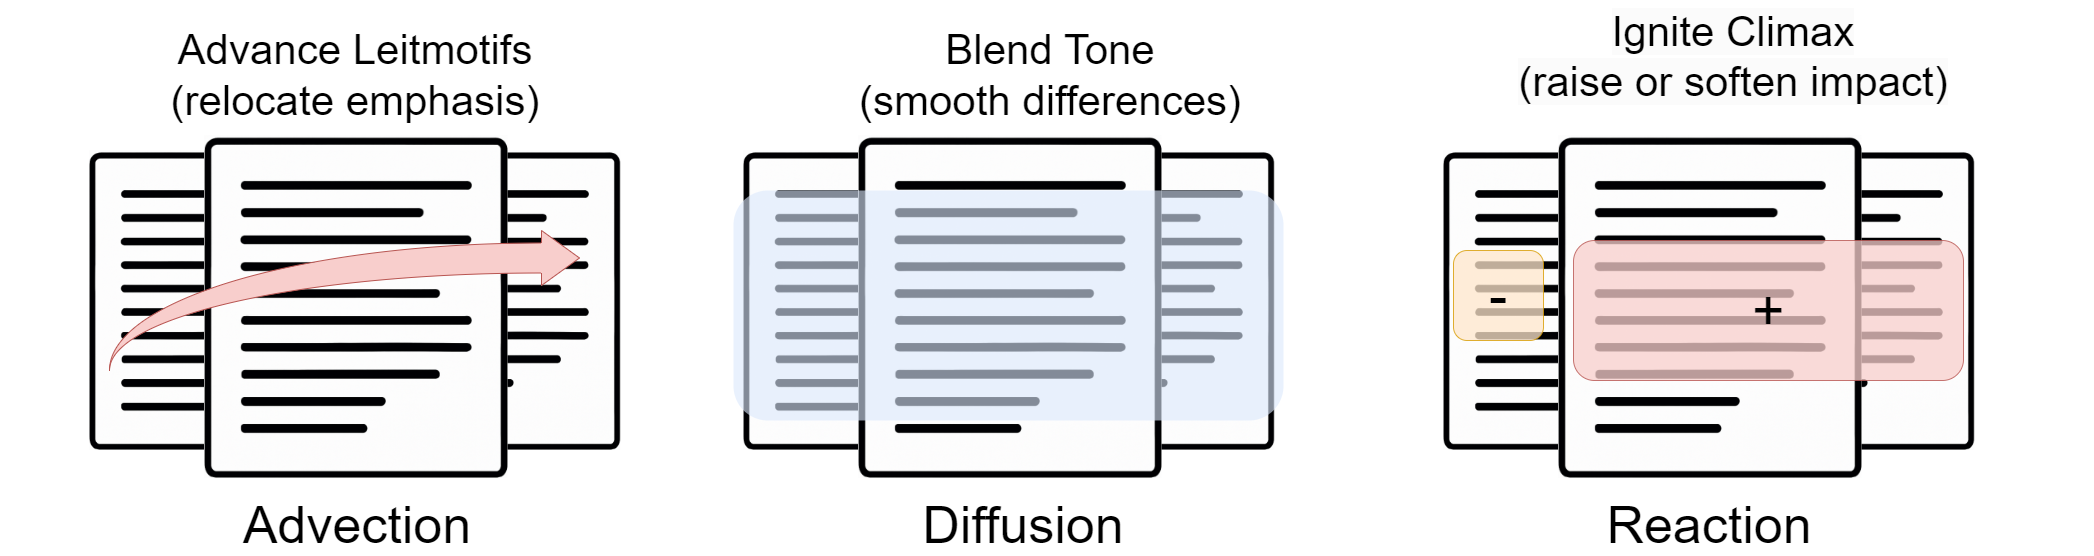
\includegraphics[width=1.0\linewidth]{figures/dar.png}
\caption{Left: Advection---a red arrow transport an emphasis (e.g., a leitmotif) from one paragraph to the next.
Center: Diffusion---A blue band envelops similar paragraphs, showing tone blending that smooths local stylistic differences.
Right: Reaction---a red overlay with $+$ mark amplified paragraphs, while an orange overlay with a $\text{-}$ mark indicates decayed paragraphs.s}
\label{fig:why}
\end{figure}

\section{Contextual and Lexical score}\label{app:lex_sem}

Given the  onotlogy $\mathrm{T} = (\mathcal{C},\mathcal{A})$,
where $\mathcal{C} = \{C_{1},\dots,C_{m}\}$ is a finite set of classes; $\mathcal{A} = \bigcup_{j=1}^{k}\mathcal{A}_{C_{j}}$ is the \emph{A-box}, with
$\mathcal{A}_{C_{j}} \;=\;
\bigl\{\,a : C_{j} \mid a \in \mathcal{I}_{C_{j}}\,\bigr\}$         where each $a\!:\!C_{j}$ asserts that individual
\(a\) instantiates class \(C_{j}\) and
\(\mathcal{I}_{C_{j}}\) is the set of such individuals. $\mathcal{A}_{\mathcal{C}_j}$ denotes the A-box fragment corresponding to class $\mathcal{C}_j$ and includes all sentences or definitions from the book that are instances of $\mathcal{C}_j$.
The lexical score is defined as follows:
\begin{equation}
s_{\text{lex}}(P_i,C_j)
= \operatorname{TF\!-\!IDF}\!\Bigl(Q_i,\;
\underbrace{\textstyle\bigoplus_{a\in\mathcal{A}_{C_j}} a}_{\text{concatenation of all }a\text{ in }\mathcal{A}_{C_j}}\Bigr),
\end{equation}

\noindent

where $\operatorname{TF-IDF}$ is the \emph{Term Frequency-Inverse Document Frequency} \cite{sparck1972statistical} computed by treating $Q_i$ as a term set and $\bigoplus_{a\in\mathcal{A}{C_j}} a$ as the single document obtained by concatenating all sentences $a\in\mathcal{A}{C_j}$; the symbol $\bigoplus$ denotes the string concatenation operator.  The contextual score is computed as shown in Eq. \ref{eq:semantic}.
\begin{equation}\label{eq:semantic}
\mathrm{Emb}(\mathcal{A}_{C_j})
= \frac{1}{|\mathcal{A}_{C_j}|}\sum_{a\in\mathcal{A}_{C_j}}\mathrm{Emb}(a), \quad
s_{\text{ctx}}(P_i,C_j)
= \cos\!\bigl(\mathrm{Emb}(P_i),\,\mathrm{Emb}(\mathcal{A}_{C_j})\bigr),
\end{equation}

\noindent

where $Emb$ is a SentenceTransformer \cite{reimers2019sentence}; $cos$ is the cosine similarity function, and $|\cdot|$ denotes the
cardinality of a set.
\section{Ontology T-box}
\label{app:appendix_onto}

Table \ref{tab:tab_onto_t} shows our manually designed ontology employed to model the Foucault's pendulum.
We used the following top-level classes: (i) \emph{Concepts}, indicating
metaphysical cores spanning multiple traditions, such as \emph{Tree of Life}; (ii)
\emph{Traditions}, denoting spiritual or cultural currents or schools through which the concepts are articulated (e.g., \emph{Kabbalah}); (iii) \emph{Languages and Codes} describe
terms used to classify or describe phenomena in a cross-cutting or critical manner (e.g., \emph{Abracadabra}); (iv) \emph{Figures and archetypes} refer to historical, mythical, or literary figures (e.g., \emph{John Dee})
Note that \emph{Abracadabra} is defined as a class. This is because, even though it looks like an assertion (an instance) in Foucault’s Pendulum, here it functions as a class-level concept—a prototype for any spell, inscription, or amulet that shares the same structure. This is a recurring theme in Foucault’s Pendulum because signs migrate, acquiring new meanings throughout the novel.

\setlength{\tabcolsep}{8.7pt}

\begin{table}[ht]
\centering
\caption{Snippet of the conceptual hierarchy used in this work.}
\label{tab:tab_onto_t}
\resizebox{0.8\textwidth}{!}{
\begin{tabular}{@{}p{0.5\textwidth}p{0.46\textwidth}@{}}
\toprule
\textbf{IRI} & \textbf{SubClassOf} \\
\midrule
Abracadabra                                 & Language or Code \\
Abulafia                                    & Language or Code \\
Afro-American Esotericism                   & Tradition        \\
Afro-Brazilian Esotericism                  & Tradition        \\
Alchemical Symbolism                        & Symbolism        \\
Alchemy                                     & Tradition        \\
Assassins Of Alamut                         & Secret Societies \\
Carbonari High Lodge                        & Secret Societies \\
Computational Esotericism                   & Tradition        \\
Concept                                     & Esoteric Ontology\\
Conspiratorial Jesuitism                    & Secret Societies \\
Cryptography                                & Language or Code \\
Deity                                       & Figure or Archetype \\
Esoteric Diagram Language                   & Language or Code \\
Esoteric Ontology                           & —                \\
Figure or Archetype                         & Concept          \\
Free masonry                                & Secret Societies \\
Gematria                                    & Language or Code \\
Gematria Concealed                          & Language or Code \\
Gnosticism                                  & Tradition        \\
Grail                                       & Symbolism        \\
Hermeticism                                 & Tradition        \\
Historical Figure                           & Figure or Archetype \\
Illuminati of Bavaria                       & Secret Societies \\
Imaginary and Invented Languages            & Language or Code \\
Initiatory Symbolism                        & Symbolism        \\
Islamic Esotericism or Sufism               & Tradition        \\
Kabbalah                                    & Tradition        \\
Language or Code                            & Concept          \\
Magic Squares                               & Language or Code \\
Mathematical and Geometric Language         & Language or Code \\
Modern Neo-Occultism                        & Tradition        \\
Mysterious Archaeology                      & Tradition        \\
Mythological Archetype                      & Figure or Archetype \\
Neoplatonism                                & Tradition        \\
Norse Symbology                             & Symbolism        \\
Occultism                                   & Tradition        \\
Pagan Symbology                             & Symbolism        \\
Philosopher's Stone                         & Symbolism        \\
Revelatory Symbolism or Epiphanies          & Symbolism        \\
Religious Symbolism                         & Symbolism        \\
Rosicrucianism                              & Secret Societies \\
Satanism and Luciferianism                  & Tradition        \\
Secret Societies                            & Concept          \\
Spiritism                                   & Tradition        \\
Symbolism                                   & Concept          \\
Synarchy                                    & Concept          \\
Telluric Currents                           & Concept          \\
Templar Esotericism                         & Tradition        \\
Tree of Life                                & Symbolism        \\
Tsefurim Concealed                          & Language or Code \\
Tsefurim Traditions                         & Language or Code \\
Unknown Superiors or Lords of the World     & Secret Societies \\
\bottomrule
\end{tabular}
}
\end{table}

\section{Named Entity Recognition}\label{app:appner}
To extract narrative parameters we employed a Named Entity Recognition (NER) model. \footnote{\url{https://huggingface.co/tomaarsen/span-marker-mbert-base-multinerd}.}
Figure \ref{fig:ner} shows an example of applying an NER model to two sentences from the book.
\begin{figure}[t]
\centering
\includegraphics[width=1.0\linewidth]{figures/ner_ex.png}
\caption{Example of named entities in some sentences of the novel.}
\label{fig:ner}
\end{figure}

\section{Experimental settings}\label{app:experimental}
We selected the hyperparameter using a greedy search strategy. Specifically, we set $\tau=0.65$, $\nu=0.015$, $\eta=10^{-6}$, $\lambda_{inj} = \lambda_{dec} = 0.03$, $\alpha=0.5$ and $r=15$. To ensure robustness, narrative parameters were selected only if they occurred more than  two times within the same paragraph. We include as \mxr{} nodes only those paragraphs whose advection-to-diffusion ratio exceeds the $55$th-percentile, and as \src{} and \snk{} nodes only those where $|\Delta|$ exceeds the $25$th percentile.
Considering the SentenceTransformers, we employed \textsf{BGE-M3}\footnote{\url{https://huggingface.co/BAAI/bge-m3}} \cite{bge-m3} for computing the sentence embeddings.

\section{Examples of paragraphs in Foucault's Pendulum}\label{app:examples}

Figure \ref{fig:par_examples} illustrates some of the paragraphs analyzed in our qualitative evaluation. Note also that our analysis is based on the Italian edition of Eco's novel.

\begin{figure}[t]
\centering
\includegraphics[angle=90,width=\textwidth,height=0.90\textheight,keepaspectratio]{figures/paragragraphs_examples.png}
\caption{Snippet of paragraphs extracted from Umberto Eco's Foucault's Pendulum. Since we used the Italian version of the book to perform our analysis, we manually translated the snippet into English.} \label{fig:par_examples}
\end{figure}

\end{document}